\section{Motivating Example}
\label{sec:example}

We now present some real world examples to motivate our approach. In particular, through these examples we demonstrate that developers often overlook the documentation. Thus, the resultant system is inconsistent with the intentions that a developer had in mind initially. We suspect the reason for this phenomena is that API documentation is often verbose and information is distributed across various
pages. For example, the PDF version of the documentation for Amazon S3 API\footnote{\url{http://awsdocs.s3.amazonaws.com/S3/latest/s3-api.pdf}} spans 278 pages. Developers do not have time and patience to go through all the documentation and miss various temporal specifications of the API, which often result in defective applications that do not follow temporal specifications. 
If we have the formal temporal specifications such kinds of defects can be detected by formal verification tools.

\begin{figure}[t]
\begin{center}
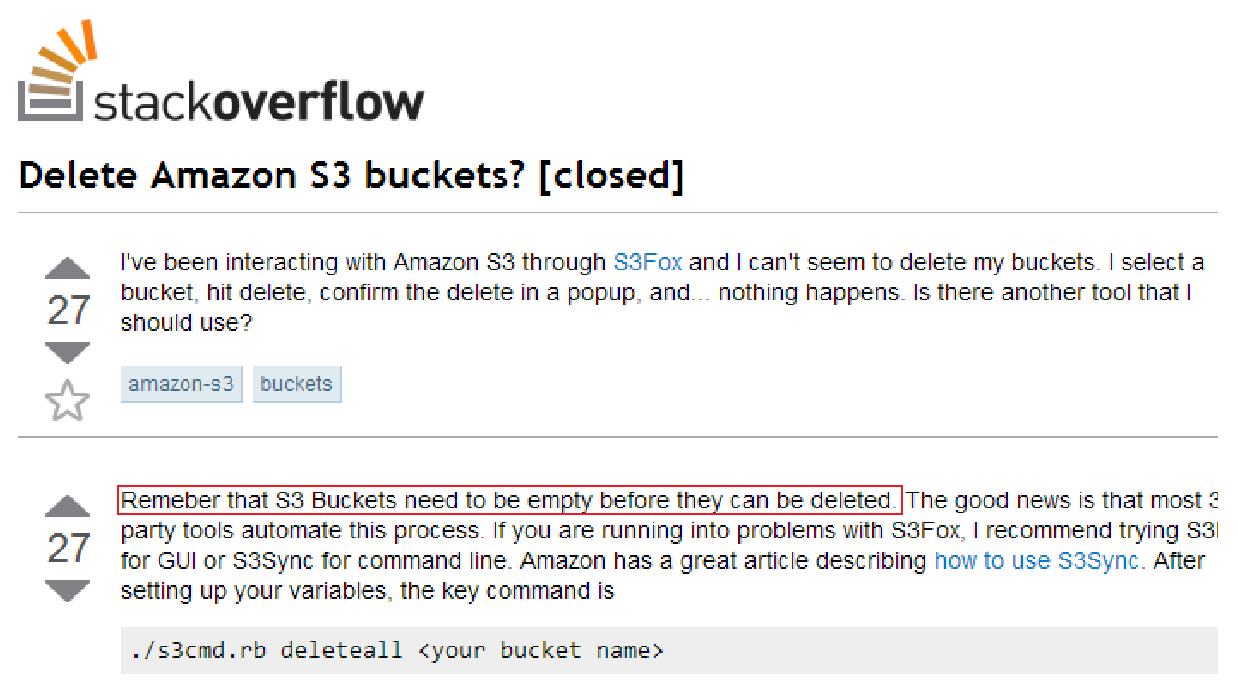
\includegraphics[scale=0.4]{Stackoverflow.eps}
\end{center}
\caption{\label{fig:Stackoverflow} The Query posted on Stackoverflow form regrading Amazon S3 REST API}
\end{figure}

Consider the question asked in \textit{Stack Overflow}~\footnote{\url{http://stackoverflow.com/}} as shown in Figure~\ref{fig:Stackoverflow}. Stack Overflow is a question and answer site for professional and enthusiast programmers. The query is about the delete functionality of a third-party software \CodeIn{S3Fox} to interact with \amazonAPI. In particular, the query complains about an issue in delete bucket functionality of the \CodeIn{S3Fox}. In particular, the issue was because the \CodeIn{S3Fox} developers overlooked the specifications in \amazon. Figure~\ref{fig:AmzonS3DeleteBucketAPI} shows the documentation of delete bucket method. The documents clearly states (outlined in red for clarity) that before deleting the bucket the objects in the buckets must be deleted. Although the issue was fixed but notice that the response on the \textit{Stack Overflow} encouraged the person asking query to switch to another product, thus potentially resulting in a loss of revenue attributed to customer dissatisfaction.  


\begin{figure}[t]
\begin{center}
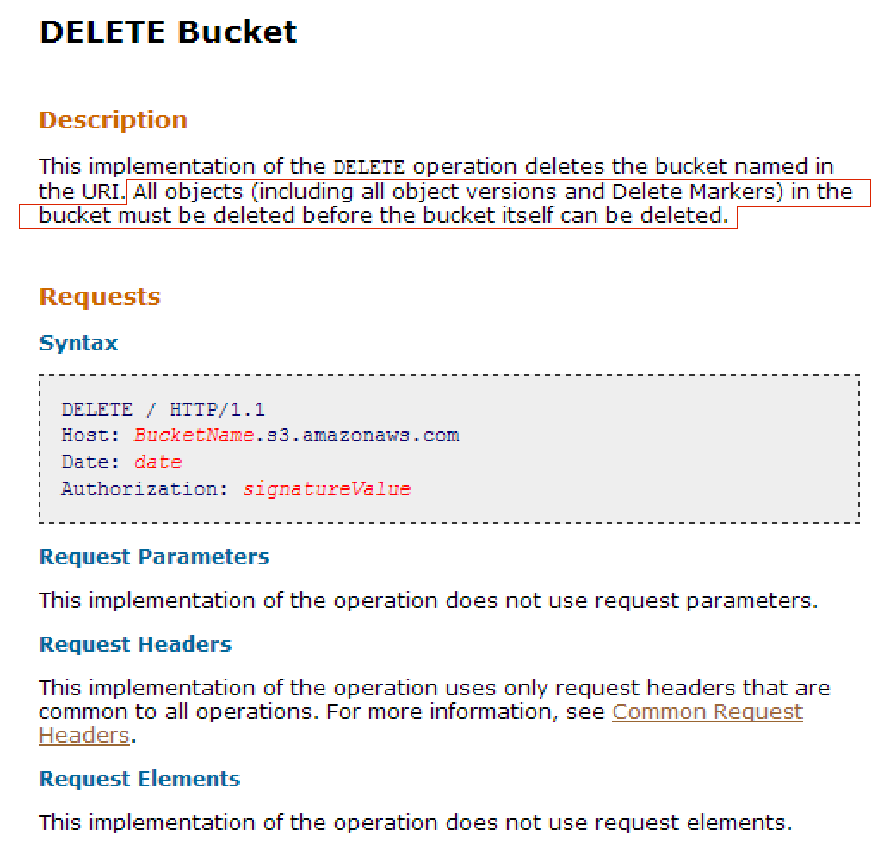
\includegraphics[scale=0.4]{AmzonS3DeleteBucketAPI.eps}
\end{center}
\caption{\label{fig:AmzonS3DeleteBucketAPI} The online API document for \CodeIn{DELETE Bucket} operation in Amazon S3 REST API}
\end{figure}


In yet another example a developer points out the financial losses he suffered because he was incorrectly using the previously described delete bucket functionality as shown in Figure~\ref{fig:example2}. The problems in the previously described examples could have been alleviated if developers paid more attention to the documentation. However, as pointed out by Novick et. al~\cite{Novick2006WDP} that developers often overlook the documentation. Furthermore, since these documents are written in natural language they cannot be subjected to machine based verification. Thus, there is need for an approach to translate the constraints described in natural language into a more formal notation. Although, we only use examples from the developer forums and blogs for \amazon\ to motivate our approach. In next section, we briefly discuss the related work in this area.


\begin{figure}[t]
\begin{center}
\includegraphics[scale=0.4]{Example2.eps}
\end{center}
\caption{\label{fig:example2} The experience article posted by a developer regarding Amazon S3 REST API}
\end{figure}


 








